\documentclass[tikz,border=20pt]{standalone}
\usetikzlibrary{positioning, arrows.meta, shadows, calc}

\begin{document}
	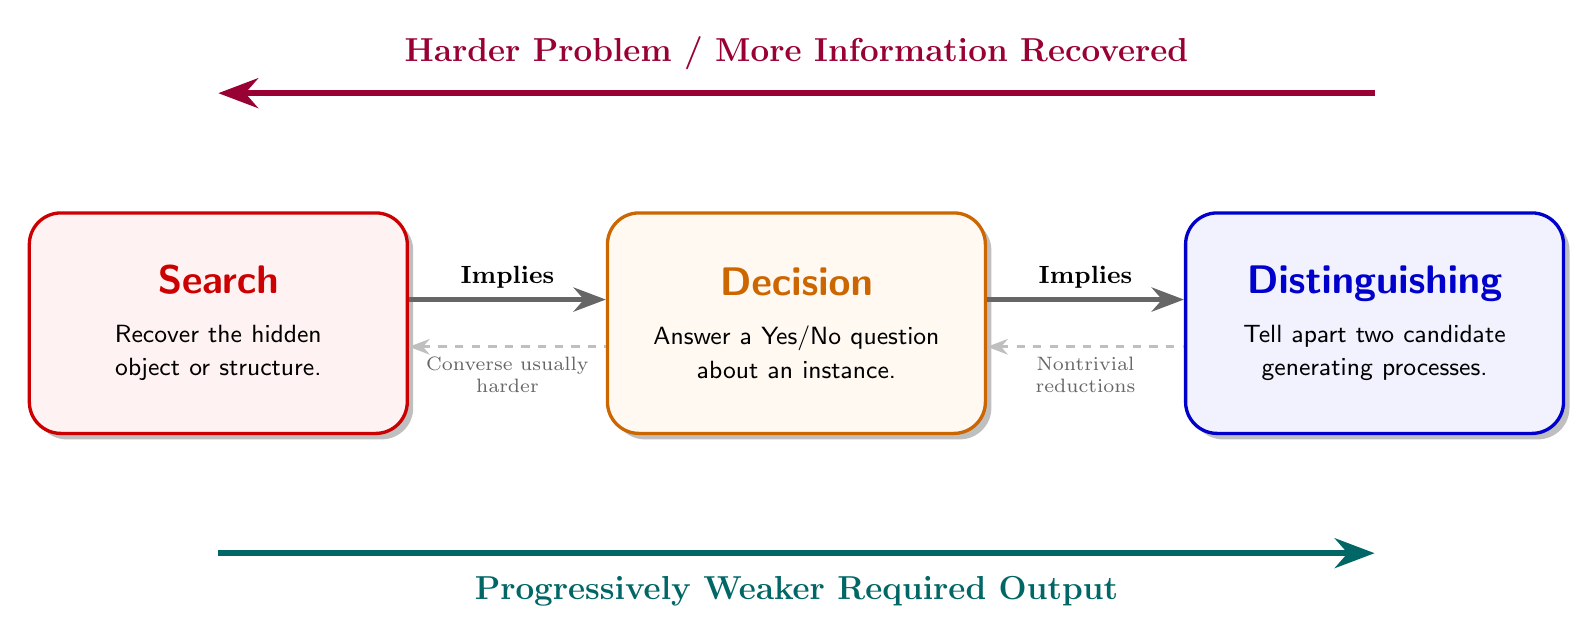
\begin{tikzpicture}[
		font=\sffamily,
		% Define styles for the boxes
		box/.style={
			rectangle, rounded corners=4mm,
			minimum width=4.8cm, minimum height=2.8cm,
			align=center, drop shadow,
			text width=4.2cm, very thick
		},
		% Specific color styles
		searchbox/.style={box, draw=red!80!black, fill=red!5},
		decisionbox/.style={box, draw=orange!80!black, fill=orange!5},
		distinguishbox/.style={box, draw=blue!80!black, fill=blue!5},
		% Arrow styles
		forwardarrow/.style={
			-{Stealth[scale=1.2]}, line width=1.5pt, draw=gray!80!black
		},
		backwardarrow/.style={
			{Stealth[scale=1.0]}-, line width=1pt, draw=gray!50, dashed
		}
		]
		
		% --- 1. Nodes representing the three problems ---
		\node[searchbox] (search) {
			{\Large\bfseries\textcolor{red!80!black}{Search}}\\[1.5ex]
			\small Recover the hidden\\object or structure.
		};
		
		\node[decisionbox, right=2.5cm of search] (decision) {
			{\Large\bfseries\textcolor{orange!80!black}{Decision}}\\[1.5ex]
			\small Answer a Yes/No question\\about an instance.
		};
		
		\node[distinguishbox, right=2.5cm of decision] (distinguish) {
			{\Large\bfseries\textcolor{blue!80!black}{Distinguishing}}\\[1.5ex]
			\small Tell apart two candidate\\generating processes.
		};
		
		% --- 2. Logical Implication Arrows (Between boxes) ---
		% Forward (Implies)
		\draw[forwardarrow] ([yshift=3mm]search.east) -- 
		node[above, font=\bfseries\small] {Implies} 
		([yshift=3mm]decision.west);
		
		\draw[forwardarrow] ([yshift=3mm]decision.east) -- 
		node[above, font=\bfseries\small] {Implies} 
		([yshift=3mm]distinguish.west);
		
		% Backward (Harder converse)
		\draw[backwardarrow] ([yshift=-3mm]search.east) -- 
		node[below, font=\scriptsize\color{gray!80!black}, align=center] {Converse usually\\harder} 
		([yshift=-3mm]decision.west);
		
		\draw[backwardarrow] ([yshift=-3mm]decision.east) -- 
		node[below, font=\scriptsize\color{gray!80!black}, align=center] {Nontrivial\\reductions} 
		([yshift=-3mm]distinguish.west);
		
		% --- 3. overarching Concept Arrows (Top and Bottom) ---
		% Top arrow: Decreasing Difficulty
		\draw[{Stealth[scale=1.2]}-, line width=2pt, draw=purple!80!black]
		([yshift=1.5cm]search.north) -- ([yshift=1.5cm]distinguish.north)
		node[midway, above=4pt, font=\large\bfseries\color{purple!80!black}] 
		{Harder Problem / More Information Recovered};
		
		% Bottom arrow: Weaker required output
		\draw[-{Stealth[scale=1.2]}, line width=2pt, draw=teal!80!black]
		([yshift=-1.5cm]search.south) -- ([yshift=-1.5cm]distinguish.south)
		node[midway, below=4pt, font=\large\bfseries\color{teal!80!black}] 
		{Progressively Weaker Required Output};
		
	\end{tikzpicture}
\end{document}